%% LyX 2.1.4 created this file.  For more info, see http://www.lyx.org/.
%% Do not edit unless you really know what you are doing.
\documentclass[oneside,english]{amsart}
\usepackage[T1]{fontenc}
\usepackage[latin9]{inputenc}
\usepackage{geometry}
\geometry{verbose}
\usepackage{float}
\usepackage{amstext}
\usepackage{amsthm}
\usepackage{cancel}
\usepackage{graphicx}

\makeatletter
%%%%%%%%%%%%%%%%%%%%%%%%%%%%%% Textclass specific LaTeX commands.
\numberwithin{equation}{section}
\numberwithin{figure}{section}

\makeatother

\usepackage{babel}
\begin{document}

\title{Red-black Tree insertion and deletion}

\maketitle

\section{Binary-Search Tree }

The ``binary-search'' invariant is that a node is greater or equal
to its left child and less than or equal to its right child.


\subsection{Insertion}

Simple: just walk down the tree going left or right depending on whether
the value you're inserting is greater or smaller than the value at
the node.


\subsection{Deletion}

Simple: if the node you're deleting only has one child just replace
it with its child. The ``binary-search'' invariant isn't violated
and you're all set. If the node you're deleting has both of its children
then you need to replace it with a node that will preserve the ``binary-search''
invariant: either its predecessor or successor\footnote{Finding the successor or predecessor is easy: go to the left child
and then go all the down the chain of right children or the obverse
go to the right child and all the way down the chain of left children.
Note the successor won't have a left child and the predecessor won't
have a right child (why?)}. The successor (or the predecessor) is deleted outright and replaced
with its appropriate child.


\section{Red-black Tree}

A Red-black tree is a Binary-search\footnote{Stolen from http://cs.wellesley.edu/\textasciitilde{}cs231/fall01/red-black.pdf}
tree that further satisfies the invariants
\begin{enumerate}
\item Every node is ``colored'' either red or black.
\item The root of the tree is black.
\item 
\item No two red nodes in a row, i.e. if a node is red then both of its
children are black.
\item Every path down from a node to a leaf should have the same number
of black nodes (called black-depth).
\end{enumerate}
A conseqeuence of satisfying these invariants is that for any node
$x$ in the tree with $n$ nodes it's the case that
\[
\lg\left(n\right)<\text{height}\left(x\right)\leq2\lg\left(n+1\right)
\]
(conventional height). In this sense a Red-black tree is balanced.


\subsection{Insertion}

Insert a red node using standard BST insertion. Which Red-black properties
could be violated? Property 1 holds since you inserted a red node.
Property 5 holds since you didn't add any black nodes. Property 2
might be violated if the node you inserted replaced the root and Property
4 might violated if you inserted underneath a red node. So work needs
to be done inorder re-assert the invariant. The rules appear in figure
\ref{fig:RB-Insertion-fix}. Note that if y's parent is red then the
fix needs to be repeating with y's grandparent (which will be black\footnote{why?}).
If you get all the way to the top and the new y, i.e. the root, is
still not black then just color it black (why is this okay?). 
\begin{figure}
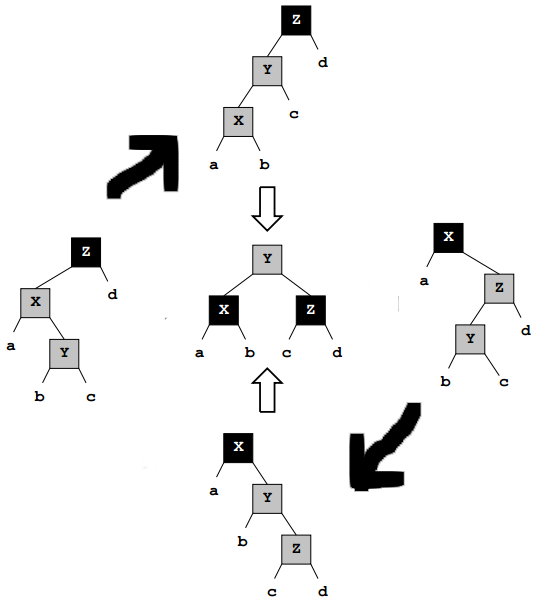
\includegraphics[scale=0.7]{rb_insert_fix}

\caption{RB Insertion fix\label{fig:RB-Insertion-fix}}


\end{figure}



\subsection{Deletion}

Use the usual BST deletion algorithm. Recall that in BST deletion
a node with only one child is replaced at some point: either the original
node has only one child (and is therefore replaced by that child)
or the original node's successor (predecessor) is replaced by its
right (left) child. Let this node (the one with only one child, by
whom it is replaced) be called $N$ and the child that moves into
$N$'s position be called $x$. It's important to keep $N$ and $x$
straight. In the case where the originally deleted node has only one
child $N$ is the original node and $x$ is the child it's replaced
with. In the case where the original node deleted is replaced by its
successor $N$ is its successor and $x$ is the successor's right
child that moves into $N$'s original position.

Which properties might be violated? If $N$ was the root and a red
node becomes the root then property 2 is violated. Otherwise if $N$'s
parent was red and $N$'s child was red then property 4 is violated
(note $N$ is necessarily black then). Finally if $N$ is black then
property 5 (black-depth) is violated by moving it up the tree (any
path that contained $N$ has one fewer black node on it now). We can
correct this by making the child $x$ that replaced $N$ be ``extra''
black. This is a bookkeeping device and no really modification to
$x$ is done. This restores property 5 but violates property 1 (what
does it mean to be ``extra'' black?). The solution is to propagate
the ``extra'' blackness up the tree according to the follow rules
until you get to the root (at which point it can just be discarded):\\

\begin{enumerate}
\item [Case A (3,4 CLRS)]: The sibling of the ``extra'' black node is
black and at least one nephew is red. This is taken care of by one
or two rotations (figure \ref{fig:Case-A-delete}; black square denotes
``extra'' blackness )
\begin{figure}[H]


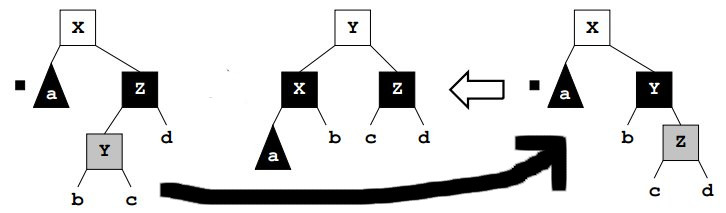
\includegraphics[scale=0.7]{rb_delete_fix_case34}\caption{Sibling black and at least one newphew red; black square denotes ``extra''
blackness fix\label{fig:Case-A-delete}}
\end{figure}

\item [Case B (2 CLRS)]: The sibling of the ``extra'' black node is black
and both nephews are black. This rule propagates the blackness up
(figure \ref{fig:Case-B-delete})
\begin{figure}[H]
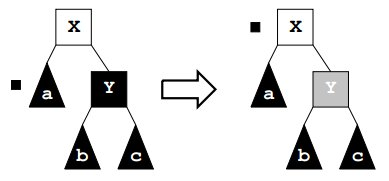
\includegraphics[scale=0.7]{rb_delete_fix_case2}\caption{Sibling black and both newphews red; black square denotes ``extra''
blackness fix\label{fig:Case-B-delete}}
\end{figure}

\item [Case C (1 CLRS)]: The sibling of the ``extra'' black node is red.
This rule transforms to either case A or B (figure \ref{fig:Case-C})
\begin{figure}[H]
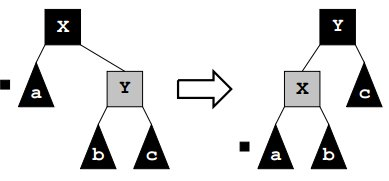
\includegraphics[scale=0.7]{rb_delete_fix_case1}\caption{Sibling red; black square denotes ``extra'' blackness fix\label{fig:Case-C}}
\end{figure}
\end{enumerate}

\end{document}
